\textbf{\underline{OZ 6 - Magnetische inductie en de wet van Faraday - Oefening 2:}}
\vspace{0.5cm}

    \begin{minipage}{.79\textwidth}
        Een cirkelvormig circuit met straal $r$ bevat een weerstand $R$ en capaciteit $C$, en
        bevindt zich in een uniform magneetveld $\vec{B}$. Startend op tijdstip $t = 0$, begint het spanningsverschil $\Delta V = V_b - V_a$ over de condensator platen toe te nemen met tijd volgens $\Delta V = V_0 (1- e^{\frac{-t}{\tau}})$, met $V_0$ en $\tau$ positieve constanten. Bepaal $\frac{dB}{dt}$, de snelheid waarmee de grootte van het magnetisch veld verandert in functie van de tijd. Wordt $B$ groter of kleiner wanneer de tijd vordert?
    \end{minipage}
    \hspace{0.3cm}\begin{minipage}{.17\textwidth}
        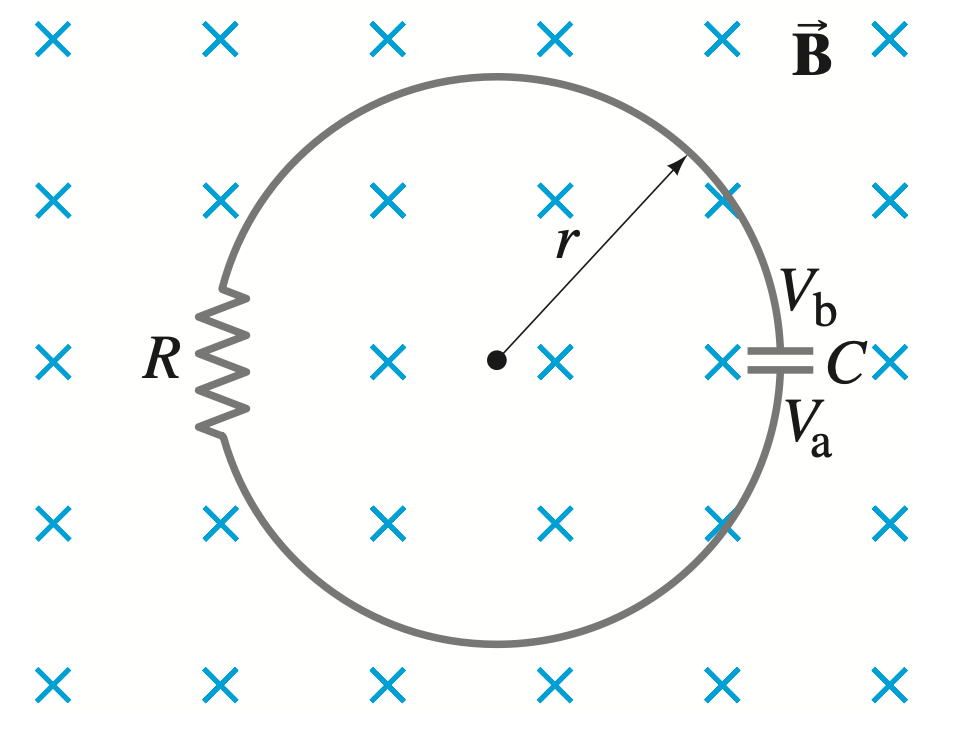
\includegraphics[scale = 0.23]{oz06/resources/Oz6Oef2.png}
    \end{minipage}

    \begin{description}[labelwidth=1.5cm, leftmargin=!]
        \item[Geg. :] $\vec{B}$, $R$, $C$, $r$, $V_0$, $\tau$
        \item[Gevr. :] $\frac{dB}{dt}$
        \item[Opl. :]
            Het magnetisch veld zal een emf induceren in het circuit, waardoor er een stroom tegen-wijzerzin zal lopen. De stroom kunnen we vinden met volgende formule 
            \begin{equation*}
                I = \frac{dQ}{dt} = \frac{d}{dt} \left(CV_0(1-e^{\frac{-t}{\tau}})\right) = \frac{V_0}{R}e^{\frac{-t}{\tau}}
            \end{equation*}
            waaruit we de geinduceerde emf kunnen vinden
            \begin{equation*}
                \mathcal{E}_{\text{ind}} = IR + V_C = V_0e^{\frac{-t}{\tau}} + V_0\left( 1 - e^{\frac{-t}{\tau}}\right) = V_0
            \end{equation*}
            wat we kunnen stoppen in de wet van faraday om de verandering van het magnetisch veld te vinden
            \begin{equation*}
                \frac{dB}{dt} = - \frac{\mathcal{E}_{\text{ind}}}{A} = - \frac{V_0}{\pi r^2}
            \end{equation*}
            en dus blijkt dat het magnetisch veld vermindert.

    \end{description}


\vspace{1cm}